% IGARSS submission. Four pages, IEEE two-column.
%
% Every number in this file was produced by a named script in the repository and
% can be traced to a JSON result file. Nothing is quoted from memory.
%   Table I        data/FINAL.json
%   Table II       data/learnable_test.json, data/eval_vs_optical.json
%   Table III      data/looks_pilot_result.json
%   Figures        data/report/*.png
\documentclass[10pt,conference]{IEEEtran}
\usepackage{graphicx,booktabs,amsmath,url,balance}
\begin{document}

\title{What Can InSAR Coherence Change Actually Label?\\
A Measured Ceiling from 617 Desert Flash Floods}

\author{\IEEEauthorblockN{Adham Ahmed}
\IEEEauthorblockA{The American University in Cairo\\
Cairo, Egypt\\
adhamahmed804@aucegypt.edu}}

\maketitle

\begin{abstract}
Coherence change detection is the usual way to label floods in SAR imagery, but
its limits are described in words rather than measured. We build a dataset of
617 desert flash floods across six arid basins. Every event is paired with a
quiet control date at the same place, the same season and the same orbit. At
event level the label works well: floods beat their own controls in 86.8\% of
174 pairs ($p = 2.8\times10^{-24}$). At pixel level it is bounded, and we
measure the bound four ways. Predicting flood extent from terrain, basin
routing and catchment routed rainfall gives AUC 0.695 on basins the model never
saw. A separately trained model with identical features, evaluated on ground it
has already seen in training, reaches 0.826. Splitting by pixel instead of by
event gives 0.926, which is spatial autocorrelation rather than skill. Scored against independent Sentinel-2 optical labels on the same pixels,
the model rises from 0.643 to 0.751. Reprocessing at sixteen times more looks
cuts label noise by a factor of 22 but does not improve agreement with the
optical evidence. We conclude that coherence responds to surface disturbance in
general, not to water in particular, and that this limits pixel scale flood
extent prediction more than model capacity does.
\end{abstract}

\begin{IEEEkeywords}
InSAR, coherence change detection, flash floods, arid regions, Sentinel-1,
flood labelling, spatial validation
\end{IEEEkeywords}

\section{Introduction}
Flash floods in dry basins are short, local and rarely gauged. They are
under-represented in flood datasets, most of which were built for large rivers.
Interferometric coherence change detection is the common way to label them from
SAR. Coherence is computed for a pair of images before the event and for a pair
that spans it, and a drop in coherence is read as flooding.

The weaknesses of this method are well known and rarely quantified. Papers list
vegetation decorrelation, revisit time and urban geometry as problems, but the
field has no measurement of how much flood extent such a label can support, or
of what the processing settings cost.

Separately, that random splits overstate accuracy on spatially structured data
is established in the wider geospatial modelling literature: block
cross-validation gives more conservative and more realistic estimates
\cite{roberts2017}, and random splits have been shown to overstate the
predictive skill of large-scale ecological maps by a wide margin
\cite{ploton2020}, though the appropriate remedy is contested
\cite{wadoux2021,meyer2022}. We do not claim this effect is new. We quantify it,
for the first time to our knowledge, on InSAR-labelled flood data, and add an
axis this literature has not: splitting by \emph{event}, since tiles from one
event are not independent even when they are not geographically close.

This paper provides that measurement. Our contributions are:

\begin{itemize}
\item a dataset of 617 InSAR labelled desert flash floods with 174 paired quiet
      control dates across six basins, a control design that is rare in flood
      mapping;
\item a measured ceiling. Within one basin, with spatial leakage removed, the
      the label is learnable to 0.675 on average (range 0.570 to 0.745), and
      our model reaches 0.695 across basins it has never seen;
\item evidence that the limit is physical rather than procedural, since more
      multilooking reduces noise but does not improve agreement with an
      independent optical label.
\end{itemize}

\section{Data}

\subsection{Events and controls}
We collect 617 flash flood events between 2015 and 2025 in six HUC4 basin
groups of the arid southwestern United States. Each event uses Sentinel-1 burst
interferometry processed by ASF HyP3 at $5\times1$ looks, giving 20\,m pixels.

Labelling uses the three scene design. A baseline pair of two pre-event scenes
shows what coherence looks like with no flood. A co-event pair spans the event.
The label is the difference between them,
$\Delta\gamma = \gamma_{\mathrm{base}} - \gamma_{\mathrm{co}}$. It is stored as
a continuous value and only turned into a yes or no at scoring time.

Each event is also paired with a \emph{quiet control}: the same burst, the same
orbit and a similar season, on a date with no flood reported. These 174 controls
let us test the label against natural decorrelation instead of assuming it.

\subsection{Predictors}
We use 30 channels, all of which are known before the event. Terrain comes from
1\,m lidar and is degraded to five resolutions from 1\,m to 30\,m, giving mean
and minimum elevation, micro-relief, roughness and slope. Basin routing gives
flow accumulation, height above nearest drainage, slope, stream power index and
topographic wetness index, all computed over the whole basin rather than the
image window. Rainfall comes from MRMS radar. We also compute
\emph{catchment routed rainfall}, in which rainfall is accumulated downhill over
the area draining into each pixel, which turns ``how much rain fell here'' into
``how much water arrives here''. Soil properties come from POLARIS and land
cover from ESA WorldCover.

\section{Method}

Tiles of $112\times112$ pixels at 20\,m, which is 2.24\,km across, are cut from
each event. Data are split by basin group and never at random. In our dataset
80\% of events lie within 5\,km of another event, so a random split puts nearly
identical terrain on both sides. We measure the effect of this in
Section~\ref{sec:ceiling}.

The model is a small U-Net with 4.4 million parameters. It has an elevation term
in the output and a head that sees several scales at once. We also train a tile
level \emph{gate}, a gradient boosted classifier that answers whether any
flooding happened anywhere in a 2.24\,km tile, and we set pixel predictions to
zero in tiles the gate calls dry.

All decision cutoffs are fitted on a held out validation basin and expressed as
a flagging \emph{rate}, that is, what fraction of pixels to mark as flood. An
absolute probability cutoff does not carry from one basin to another because
score distributions differ, while a rate does.

\section{Results}

\subsection{Prediction performance}
Table~\ref{tab:main} gives held out performance. Ranking pixels by elevation
alone, which needs no training and no rainfall, gives AUC 0.480. The model
reaches 0.695, and adding the gate brings it to 0.739. Scoring in 160\,m cells,
where each cell averages 64 label pixels, gives 0.757.

\begin{table}[t]
\caption{Held out basins. Cutoff fitted on validation.}
\label{tab:main}
\centering
\begin{tabular}{lcccc}
\toprule
Predictor & AUC & Recall & Precision & F1 \\
\midrule
Elevation rule, 20\,m          & 0.480 & 0.601 & 0.053 & 0.097 \\
Model, 20\,m                   & 0.695 & 0.397 & 0.101 & 0.162 \\
Model + gate, 20\,m            & 0.739 & 0.498 & 0.127 & 0.203 \\
Model, 160\,m cells            & 0.710 & 0.446 & 0.132 & 0.204 \\
\textbf{Model + gate, 160\,m}  & \textbf{0.757} & \textbf{0.533} & \textbf{0.158} & \textbf{0.244} \\
\bottomrule
\end{tabular}
\end{table}

The gate is worth 0.046 AUC and removes 76\% of false alarms. A bootstrap over
events puts the 20\,m model at 0.695 with a 95\% interval of 0.647 to 0.741.

Two caveats belong with that number. First, it is the highest of 21 comparable
configurations whose median is 0.679, so it is optimistic even though nothing
was tuned on the test set. Second, three runs of the identical configuration,
differing only in random seed, span 0.659 to 0.710. Differences below about 0.05
between configurations are therefore not distinguishable, and the honest summary
of our model is $0.68 \pm 0.03$. Notably, terrain alone reaches 0.745 on this
metric while being unable to separate flood days from quiet days at all (0.508
against 0.798 for the full model), so feature choice trades one capability for
the other rather than improving both.
Across six leave one basin out folds the model beats the elevation rule in five;
the smallest basin, with 436 tiles, falls to chance.

Catchment routed rainfall is the strongest single predictor. A gradient boosted
tree trained on the same features independently ranks routed runoff depth first
by gain, which is useful confirmation from a different model family.

\subsection{Where the limit is}
\label{sec:ceiling}
Table~\ref{tab:ceiling} locates the limit in the label rather than the model.

\begin{table}[t]
\caption{Four measurements of the ceiling.}
\label{tab:ceiling}
\centering
\begin{tabular}{lc}
\toprule
Measurement & AUC \\
\midrule
Split by pixel, mean of six basins (leakage) & 0.926 \\
Split by event, one basin (mean of six)     & 0.675 \\
Our model, unseen basins                    & 0.695 \\
Shuffled label control                      & 0.501 \\
\midrule
Model graded by InSAR label                 & 0.643 \\
Model graded by Sentinel-2 optical label    & 0.751 \\
\bottomrule
\end{tabular}
\end{table}

\emph{Learnability.} Splitting by event inside a single basin removes the need
to generalise while keeping the evaluation pixels unseen. Across all six basins
this gives a mean of 0.675, ranging from 0.570 to 0.745, with a shuffled label
control at 0.500 confirming the test is sound. We do not read this as a ceiling,
because the within basin test trains on half the events of one basin while the
full model trains on five, so it is confounded by training set size. Splitting by
\emph{pixel} instead gives 0.926 (mean of six basins), because a pixel and its neighbour 20\,m away
end up on opposite sides of the split. That comparison is not confounded, since
both sides use identical training data. The direction and rough size of this
effect match prior findings in ecological mapping \cite{ploton2020}; our
contribution is measuring it for InSAR flood labelling specifically, where it
had not been quantified, and showing that event identity, not only geographic
distance, drives part of the leakage.

\emph{Independent labels.} Scored against Sentinel-2 optical flood maps on the
same 6.9 million pixels, the same model weights give 0.751 instead of 0.643.
The two labels agree on only 10\,921 pixels, while coherence marks 400\,362
pixels as flooded and the optical evidence marks 19\,264.

\emph{Model family.} A gradient boosted tree that sees one pixel at a time
performs close to a U-Net that sees 2.24\,km of context, and removing every
routed basin feature costs only 0.008 AUC. Fifteen further variants, covering
terrain resolution, loss function, label threshold and class weighting, all land
within noise of each other.

\emph{Processing.} Table~\ref{tab:looks} reports a pilot in which 40 events were
reprocessed at more looks. The noise on $\Delta\gamma$ falls from 0.045 to
0.002, so a three sigma criterion goes from firing on no pixels at all to firing
on 40.5\% of them. Agreement with the optical label nonetheless falls. More
looks measure surface disturbance more precisely. They do not make it water.

\begin{table}[t]
\caption{Reprocessing 40 events at more looks.}
\label{tab:looks}
\centering
\begin{tabular}{lcccc}
\toprule
Looks & Pixel & Noise on $\Delta\gamma$ & $3\sigma$ fires on & Optical agr. \\
\midrule
$5\times1$  & 20\,m & 0.0447 & 0.00\%  & 0.631 \\
$10\times2$ & 40\,m & 0.0102 & 8.63\%  & 0.630 \\
$20\times4$ & 80\,m & 0.0020 & 40.53\% & 0.584 \\
\bottomrule
\end{tabular}
\end{table}

We also tested whether the noise is isolated speckle that could be filtered out.
Removing connected flood patches smaller than 32 pixels deletes 30\% of flood
pixels and reduces agreement with the optical label from 0.615 to 0.604. The
noise is therefore not isolated. It is connected patches in the wrong places,
which no spatial filter can separate from real flooding.

\subsection{Seen and unseen ground}
Fig.~\ref{fig:random} and Fig.~\ref{fig:region} compare two models trained with
identical features on identical tiles, one with a region split and one with a
random split, so ground appears in both its own training set and its own test
set. On seen ground the model produces a usable map, with recall 0.48 and
precision 0.39. On unseen basins the prediction still follows drainage correctly
but flags far more area than flooded, with precision 0.10. The gap of 0.131 in
AUC between the two (0.826 against 0.695) is the cost of honest spatial
validation.

\begin{figure}[t]
\centering
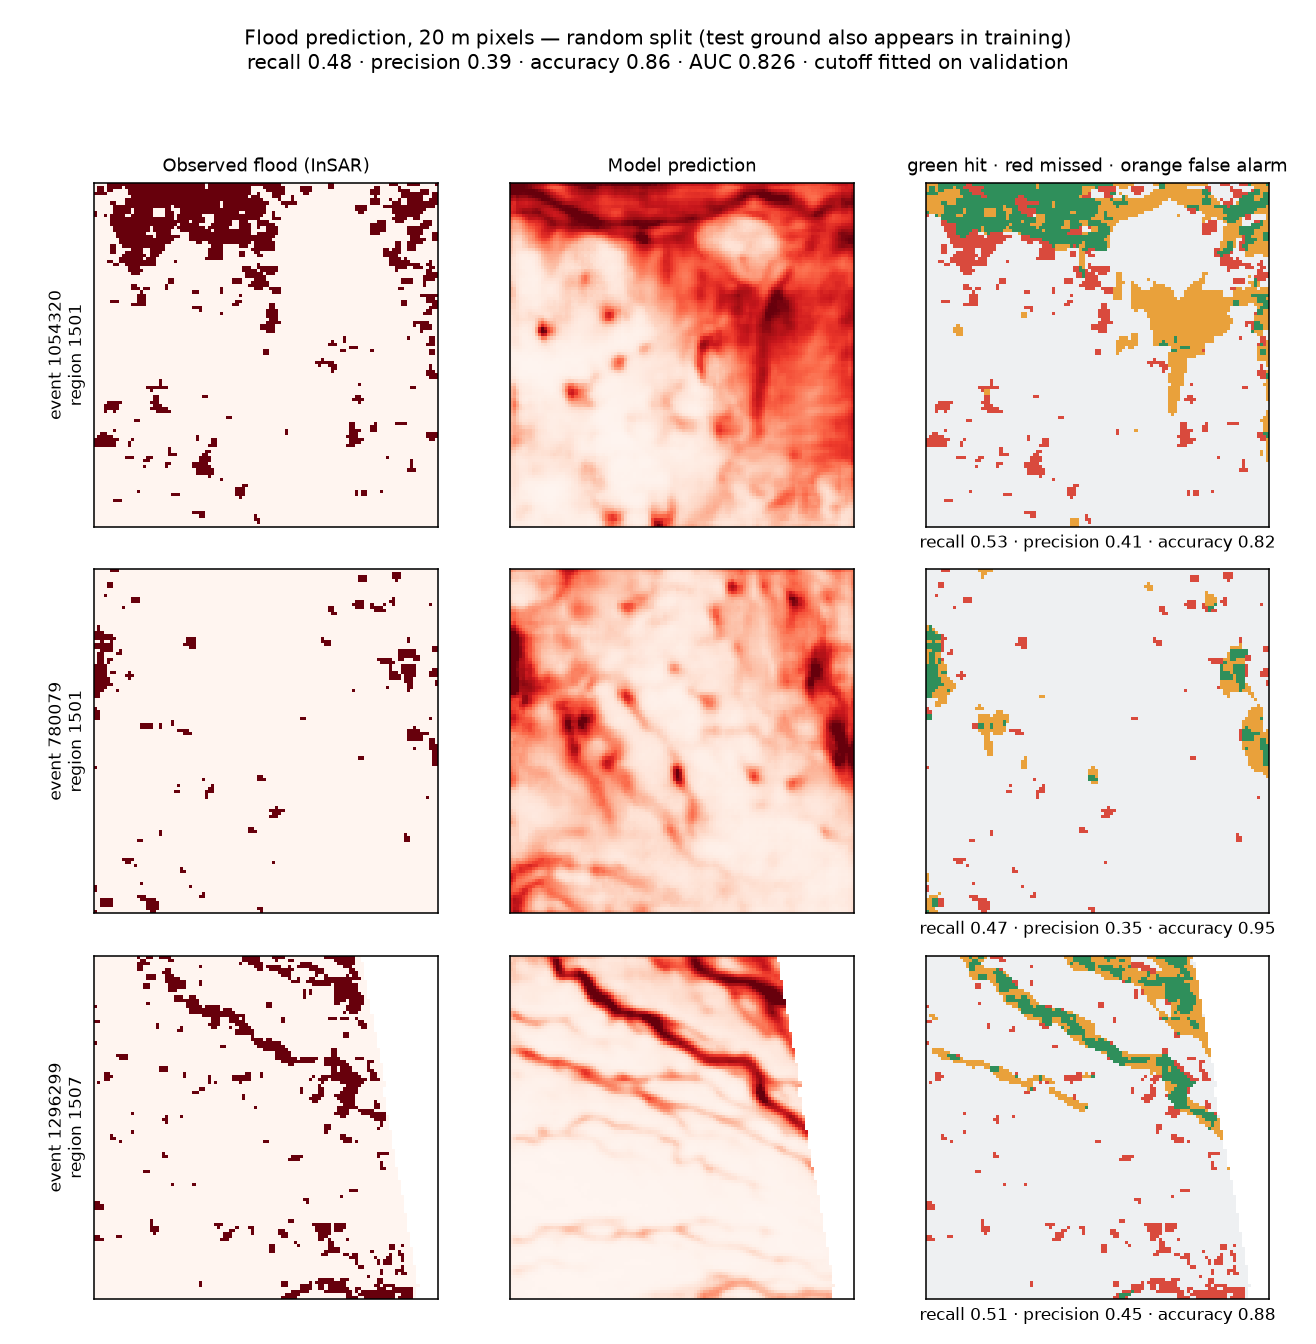
\includegraphics[width=\columnwidth]{figures/fig_random.png}
\caption{A separately trained model, identical features and tiles to
Fig.~\ref{fig:region}, evaluated with a random split so test ground also
appears in training. Recall 0.48, precision 0.39, accuracy 0.86, AUC 0.826.
This is within-basin performance and is not a transfer result.}
\label{fig:random}
\end{figure}

\begin{figure}[t]
\centering
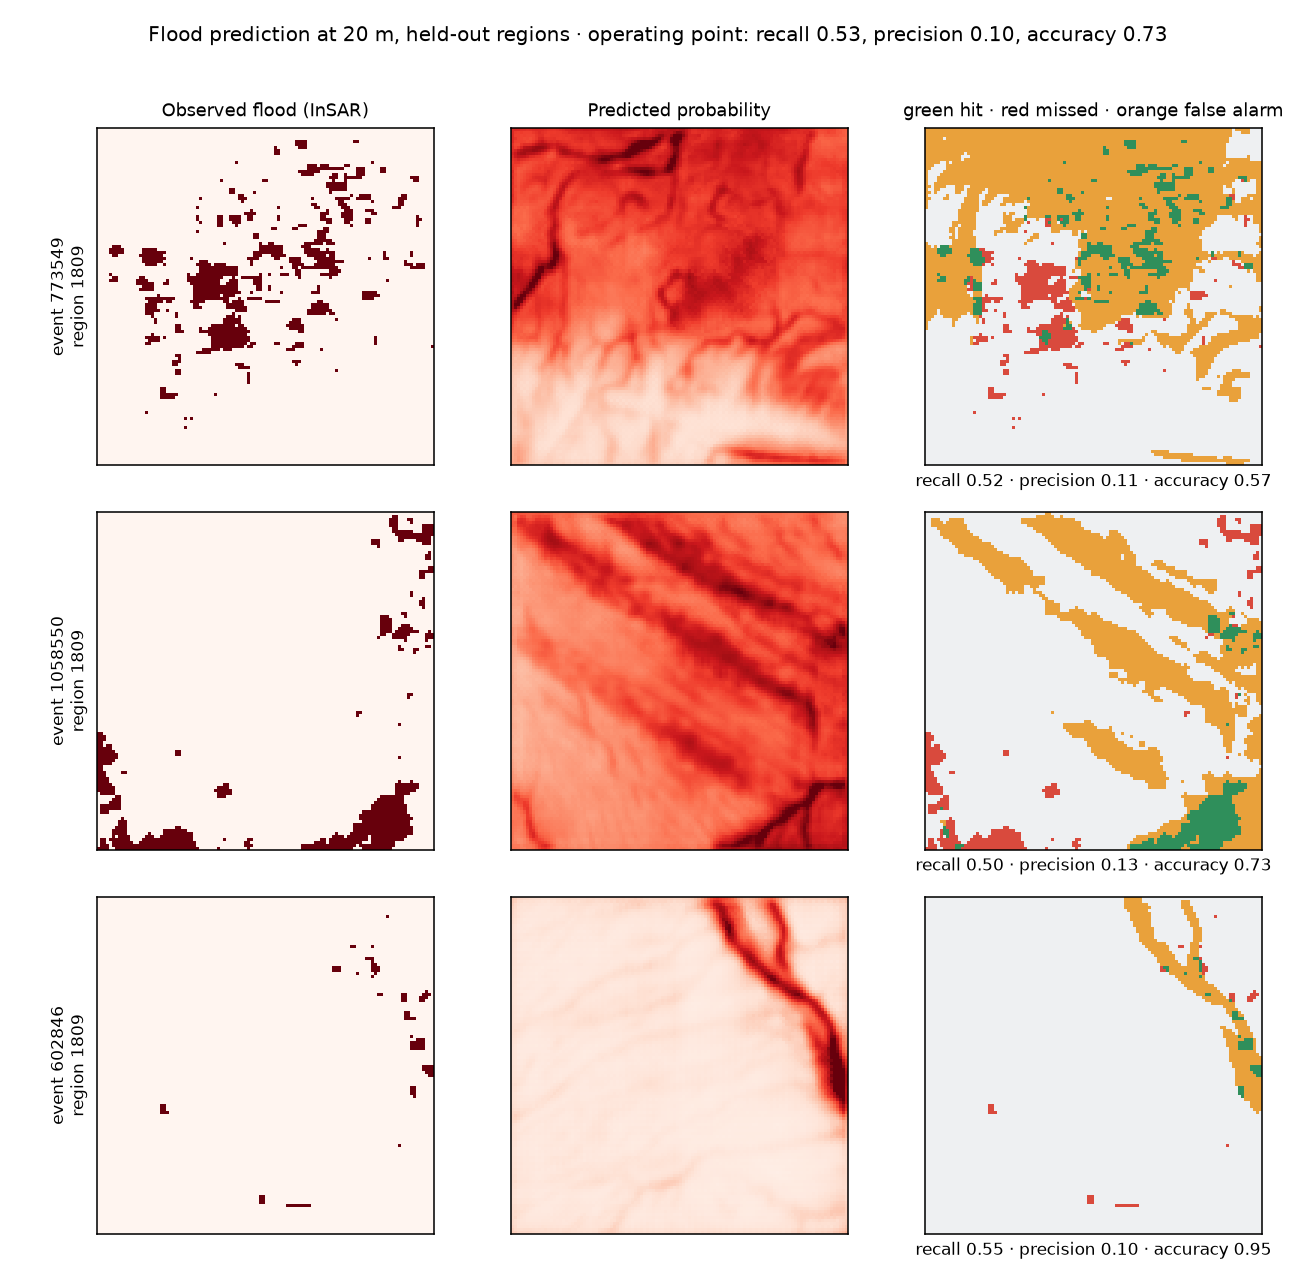
\includegraphics[width=\columnwidth]{figures/fig_region.png}
\caption{The same model on basins it never saw. Recall 0.53, precision 0.10,
accuracy 0.73. The prediction follows drainage but marks about ten times more
area than flooded.}
\label{fig:region}
\end{figure}

\begin{figure}[t]
\centering
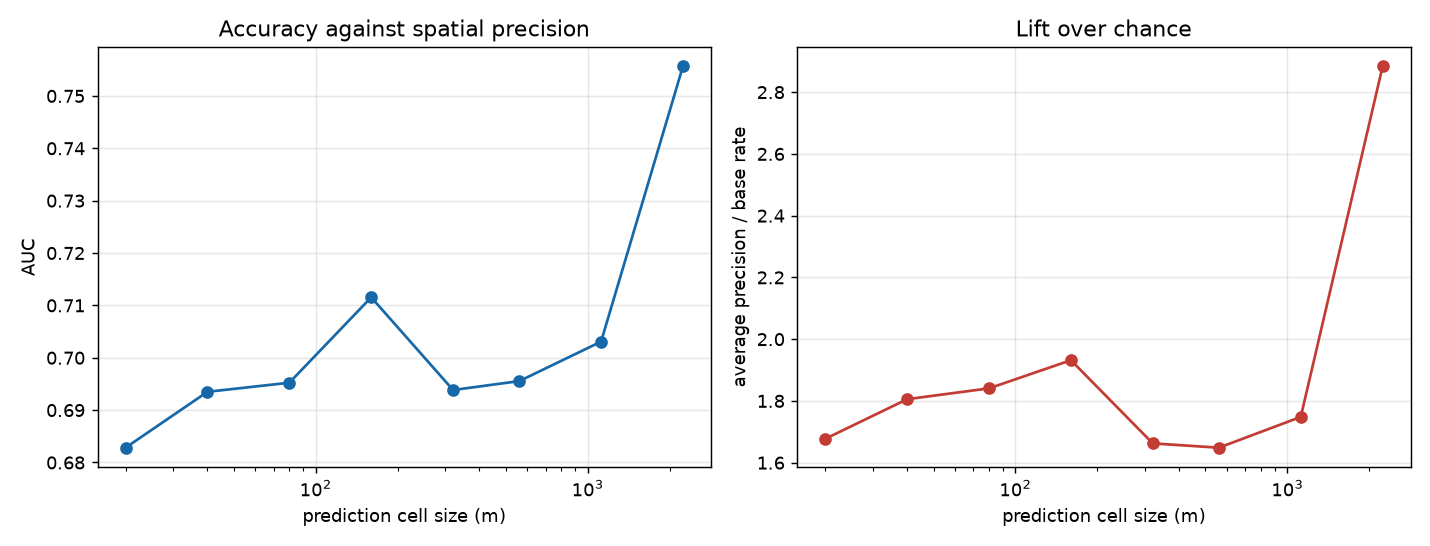
\includegraphics[width=\columnwidth]{figures/fig_scale.png}
\caption{Accuracy against the size of the prediction cell. Aggregating to 160\,m
recovers most of the achievable signal while keeping cells small enough to be
useful. Lift is average precision divided by the base rate.}
\label{fig:scale}
\end{figure}

\section{Discussion and Conclusion}
Coherence change reliably detects that a flood happened. Floods beat their own
quiet controls in 86.8\% of 174 paired comparisons. It does not reliably show
where the water went. Our evidence is that the reason is physical. Coherence
falls for any surface change, and in dry basins wind, moving sediment and
farming all contribute. Tiles containing cropland show three times the apparent
flood rate, which fits tillage rather than inundation.

For practice we suggest three things. Treat coherence derived flood extent as a
hazard ranking rather than a flood map. Validate with spatially blocked splits,
because a random split inflated our own result by 0.135 AUC and a pixel split by
0.231. Do not expect extra multilooking to recover pixel scale accuracy, since
we paid for that experiment and it did not.

The dataset, the paired controls and the code are released so that others can
measure against the same ceiling.

\section*{Acknowledgment}
Sentinel-1 and Sentinel-2 data courtesy of ESA. InSAR products generated by ASF
HyP3.

\balance
\begin{thebibliography}{9}
\bibitem{hyp3} Alaska Satellite Facility, ``HyP3 Sentinel-1 Burst InSAR
Product Guide,'' ASF DAAC, 2024. [Online]. Available:
https://hyp3-docs.asf.alaska.edu/guides/burst\_insar\_product\_guide/
\bibitem{unspider} UN-SPIDER Knowledge Portal, ``Recommended Practice: Flood
Mapping with Sentinel-1 Interferometric Coherence.'' [Online]. Available:
https://un-spider.org/advisory-support/recommended-practices/recommended-practice-flood-mapping-sentinel-1
\bibitem{polaris} N. W. Chaney, B. Minasny, J. D. Herman, T. W. Nauman,
C. W. Brungard, C. L. S. Morgan, A. B. McBratney, E. F. Wood, and
B. Yimam, ``POLARIS soil properties: 30-m probabilistic maps of soil
properties over the contiguous United States,'' \emph{Water Resour. Res.},
vol. 55, no. 4, pp. 2916--2938, 2019, doi: 10.1029/2018WR022797.
\bibitem{worldcover} D. Zanaga, R. Van De Kerchove, D. Daems, W. De
Keersmaecker, C. Brockmann, G. Kirches, J. Wevers, O. Cartus, M. Santoro,
S. Fritz, M. Lesiv, M. Herold, N. E. Tsendbazar, P. Xu, F. Ramoino, and
O. Arino, ``ESA WorldCover 10 m 2021 v200,'' 2022, doi:
10.5281/zenodo.7254221.
\bibitem{roberts2017} D. R. Roberts, V. Bahn, S. Ciuti, M. S. Boyce,
J. Elith, G. Guillera-Arroita, S. Hauenstein, J. J. Lahoz-Monfort,
B. Schr\"oder, W. Thuiller, D. I. Warton, B. A. Wintle, F. Hartig, and
C. F. Dormann, ``Cross-validation strategies for data with temporal,
spatial, hierarchical, or phylogenetic structure,'' \emph{Ecography}, vol. 40,
no. 8, pp. 913--929, 2017.
\bibitem{ploton2020} P. Ploton, F. Mortier, M. R\'ejou-M\'echain, N. Barbier,
N. Picard, V. Rossi, C. Dormann, G. Cornu, G. Viennois, N. Bayol, A. Lyapustin,
S. Gourlet-Fleury, and R. P\'elissier, ``Spatial validation reveals poor
predictive performance of large-scale ecological mapping models,''
\emph{Nature Communications}, vol. 11, art. 4540, 2020.
\bibitem{wadoux2021} A. M. J.-C. Wadoux, G. B. M. Heuvelink, S. de Bruin, and
D. J. Brus, ``Spatial cross-validation is not the right way to evaluate map
accuracy,'' \emph{Ecological Modelling}, vol. 457, art. 109692, 2021.
\bibitem{meyer2022} H. Meyer and E. Pebesma, ``Machine learning-based global
maps of ecological variables and the challenge of assessing them,''
\emph{Nature Communications}, vol. 13, art. 2208, 2022.
\end{thebibliography}

\end{document}
